\documentclass[12pt,letterpaper]{lsuetd}

%fix margins
\setlength{\topmargin}{-0.5in}
\setlength{\textheight}{9.0in}
\addtolength{\evensidemargin}{-0.50in}
\addtolength{\oddsidemargin}{-0.50in}
\addtolength{\textwidth}{1.00in}
\setlength{\parindent}{1.75em}
\setlength{\parskip}{0ex}
%
% included packages
\usepackage{amsmath} % for math
\usepackage{amssymb} % for symbols
\usepackage{setspace} % for doublespacing and singlespacing
\usepackage{graphicx} % for including graphics
\usepackage[hidelinks, bookmarksopen=false,bookmarks=false]{hyperref} % for hyperlinks
\usepackage{subcaption} % for two figures in 1
\usepackage{caption} % replace Figure 1: with Figure 1.
\usepackage{booktabs}% for booktables
\captionsetup[table]{labelsep=period}
\captionsetup[figure]{labelsep=period}
\captionsetup[lstlisting]{labelsep=period}
\usepackage{titlesec} % alternative section title, add . after the title in sections
\titlelabel{\thetitle.\quad}
\usepackage{cite} % for citations
\usepackage{soul} % for highliting
\usepackage{upgreek} %for making mu symbol not italic
\usepackage{tikz} % for figures
\usetikzlibrary{positioning, shapes} % for shapes
%
% select the fonts here
\usepackage[T1]{fontenc}
\usepackage[scaled=0.95]{inconsolata} % typewriter font
%\usepackage{gentium} 
%
%
\usepackage{xcolor} % use colors for todo
\newcommand\todo[1]{\texttt{\textcolor{red}{TODO:#1}}} %for todo
%
\usepackage{textcomp} %for copyright symbol
\usepackage{pdfpages} %for importing external pdfs
\usepackage{url} % for urls
\usepackage[hang,flushmargin]{footmisc} %dont indent footnotes
%
%%%%%%%%%%%%%%%%%%%%%%%%%%%%%%%%%%%%%%%%%%%%%%%%%%%%%%

%remove extra gap in itemize
\usepackage{enumitem}
\setitemize{noitemsep,topsep=0pt,parsep=0pt,partopsep=0pt}

\newcommand\blfootnote[1]{%
	\begingroup
	\renewcommand\thefootnote{}\footnote{#1}%
	\addtocounter{footnote}{-1}%
	\endgroup
}

\makeatletter
\renewcommand\Huge{\@setfontsize\Huge{16pt}{18}} %Redefined for use in dissertation title
\renewcommand\huge{\@setfontsize\huge{14pt}{18}} % Redefined for use in chapter titles
\renewcommand\Large{\@setfontsize\Large{12pt}{18}} % Redefined for use in section titles
\renewcommand\large{\@setfontsize\large{12pt}{18}} % Redefined for use in subsection titles
\renewcommand{\baselinestretch}{1.5}


\begin{document}
\renewcommand\@pnumwidth{1.55em}
\renewcommand\@tocrmarg{9.55em}
\renewcommand*\l@chapter{\@dottedtocline{0}{1.5em}{2.3em}}
\renewcommand*\l@figure{\@dottedtocline{1}{0em}{3.1em}}
\let\l@table\l@figure
%
\pagenumbering{roman}

% %%%%The front page %%%%%
%
\thispagestyle{empty}
\begin{center}
{\Huge \bfseries
\uppercase{Extending Distributed Functionality in Phylanx}
}


\vfill
\doublespacing
A Dissertation \\
\singlespacing
Submitted to the Graduate Faculty of the \\
Louisiana State University and \\
Agricultural and Mechanical College \\
in partial fulfillment of the \\
requirements for the degree of \\
Master of Science \\
\doublespacing
in \\

The Department of Computer Science and Engineering \\
\singlespacing
\vfill

by \\
Maxwell Reeser \\
B.S., Louisiana State University, 2018 \\
February 2020
\end{center}
\pagebreak
 %%%%End of the front page %%%%%
%
%
%
%% Add Acknowledgement in the final version
\chapter*{Acknowledgments}
\doublespacing
\vspace{0.55ex}
\label{acknowledgement}
\paragraph{}
I would like to thank many people for their help over the years in teaching me about the HPX system, C++, software development, many other aspects of producing quality research, as well as how to be a good human. First of all I am indebted to my parents for inculcating in me an appreciation for learning, hard work, and beauty in the arts. I also would like to thank the many teachers, like Mrs. Breaux, Mrs. Jones, and Ms. Cain, who, when I was younger, took an interest in my future, even when I lacked vision for what that future could be. I would like to thank Dr. Dennis Castleberry for igniting my interest in software, and opening a door into a fascinating world full of difficult problems which provides not only the opportunity for satisfying work, but the opportunity to benefit others by its fruit. I would like to also thank Dr. Samuel Kellar, Dr. Bibek Wagle, and Adrian Lemoine for teaching me about HPX and C++ which, while never formally being their responsibility, they were always more than happy to do. Last, but certainly not least, I would like to thank Dr. Hartmut Kaiser, my mentor and friend, for taking an interest in my development as a software developer and researcher, and who was willing to give me a chance to continue my studies in the Master's program knowing that I would benefit from my involvement at CCT and the Ste||ar Group far more than he, or the Ste||ar Group, ever would.

%Make sure there is one blank line at the end of the Acknowledgments text.

%
%The code below adds the Acknowledgments section to the Table of Contents.
\addcontentsline{toc}{chapter}{\hspace{-1.5em} {Acknowledgements}}
\addtocontents{toc}{\vspace{12pt}}
\pagebreak
\singlespacing
\setcounter{tocdepth}{1}
\tableofcontents
\pagebreak
%%The code below generates the List of Tables and adds it to the Table of Contents.
\renewcommand\@pnumwidth{1.55em}
\renewcommand\@tocrmarg{8.55em}
\addcontentsline{toc}{chapter}{\hspace{-1.5em} {List of Tables}}
\addtocontents{toc}{\vspace{12pt}}
\singlespacing
\listoftables
\pagebreak
%%The code below generates the List of Figures and adds it to the Table of Contents.
\addcontentsline{toc}{chapter}{\hspace{-1.5em} {List of Figures}}
\addtocontents{toc}{\vspace{12pt}}
\singlespacing
\listoffigures
\pagebreak
%The code below adds the Abstract and places it within the Table of Contents.
\renewenvironment{abstract}{{\hspace{-2.2em} \huge \textbf{\abstractname}}}{\pagebreak}
\addcontentsline{toc}{chapter}{\hspace{-1.5em} {Abstract}}
\begin{abstract}
\vspace{0.55ex}
\doublespacing
\label{abstract}
%350 word limit

The Phylanx Distributed Array Processing toolkit is a project being undertaken by the Ste||ar Group at LSU, built using the HPX runtime. This system has many single-node functions implemented, but before we started this project it had very few distributed primitives implemented. Because of matrix multiplication's foundational importance in machine learning algorithms, we chose it as our first major foray into distributed functionality. In order to provide options to users, we chose to implement two different algorithms, a tiling ambivalent one, as well as Cannon’s algorithm. We found that in a single node distributed test, both of our algorithms outperformed the serial version.

%Make sure there is one blank line at the end of the Acknowledgments text.

\end{abstract}
%%%
\pagenumbering{arabic}
\addtocontents{toc}{\vspace{12pt} \hspace{-1.8em} Chapter \vspace{-1em}}
\singlespacing
\setlength{\textfloatsep}{12pt plus 2pt minus 2pt}
\setlength{\intextsep}{6pt plus 2pt minus 2pt}
% \setlength{\parindent}{0pt} %do not indent paragraphs
% Chapters are added here
\chapter{Introduction}
\doublespacing
%

\label{chap:intro}
Introduction Chapter.

%

\pagebreak
\singlespacing
%%
%%
\chapter{Background}
\doublespacing
\label{chap:background}
\section{Motivation}

\paragraph{}
In recent years there have been several organizations which amass extremely large datasets. Whether this is browsing data from Amazon, industrial IoT sensor feedback, agricultural data sources, or self-driving car input data, there are some applications for which extremely large amounts of data can be analyzed for a variety of benefits. For certain of these applications, it is necessary to perform operations over the entire dataset at once. Examples of this include training the model for Tesla's self-driving cars, or Amazon or Netflix performing a matrix factorization on transaction or rating data. These examples and more make extensive use of linear algebra operations. Linear algebra libraries have a long history of being tuned to get optimum performance on single machines and in distributed environments using MPI, but the particular use-case of distributed linear algebra in systems like HPX\footnote{HPX is what is known as an Asynchronous Many Task (AMT) runtime}, does not have libraries that are as well-standardized.
\paragraph{}
One example which may help us understand the need for a system like Phylanx is Linear Regression\footnote{For those who are unfamiliar with the goals of linear regression, please refer to Appendix I}. In order to get a set of weights for the coefficients in a linear predictor system with one dependent variable you must solve the following linear algebra problem.
$$A^{T}Ax = A^{T}b+\epsilon$$
\paragraph{}
Depending on the application, the amount of data involved in a computation like this could be extremely large. For example, with the average person checking their phone 80 times per day, if 2 of those check-ins included use of Facebook, Facebook could get, conservatively, 100 million tcp requests from the United States every day. If, for example, they wanted to test latency on connections based on location they could easily muster a dataset of one billion network requests. Trying to perform an ordinary least-squares (OLS) regression on a dataset with a billion rows on a single node would take a very long time, but if they could distribute that application, something they could do easily with services like Amazon Web Services (AWS) or Microsoft's Azure, they could get the result back in much less time. Less time spent waiting on models being run translates to higher efficiency for analytics staff, and higher productivity.
\paragraph{}
Large linear algebra intensive computations using HPC systems are common in areas like Astrophysics, or meteorology, but less common in the machine-learning community. Most of the code bases which solve these large problems are tailor made for the particular problem using performant languages like C/C++ and Fortran, and often link to CUDA code for GPU acceleration. One of the problems then with extending the availability of HPC to ML researchers is the steep learning curve for developing distributed applications in these lower-level languages. Our goal with Phylanx then, is to provide them with a more familiar, more user-friendly API, which under the hood can take advantage of HPC resources automatically. Rather than create a separate standard, we chose to emulate the NumPy API for our front-end, since NumPy is the most commonly used library in Python, especially for Machine Learning practitioners.
\section{Matrix Multiplication}
\paragraph{}
In the above example of linear regression it is obvious that the matrix multiplication operation is an important part of the computation. Not only is this the case in linear regression, matrix multiplication is a very common element of Machine Learning algorithms in general. As a result of matrix multiplication's great importance for our target audience, we decided to focus our initial efforts for developing distributed functionality on exposing a distributed matrix multiplication operation. However, in order to better serve our goals with optimizing tiling we have implemented two different algorithms. One, what we are calling dot\_d, is extremely flexible when it comes to the tiling, such that it searches for the parts of the tiles in the RHS of the operation which overlap with the relevant dimensions for the local tile of the LHS operand. The other is a modification of Cannon's algorithm, an algorithm for distributed matrix multiplication first developed by Lynn Elliot Cannon in 1969.

\section{Background}
\paragraph{}
For the algorithms we implemented, we relied on previous work on distributed data structures in HPX by Wei et al \cite{WeiDistObj}, work on tiling by Huang et al \cite{Spartan}, much work done on the HPX system by Heller et al \cite{Heller2017}, and work on annotations in Phylanx by Hartmut Kaiser.
\subsection{Distributed Object}

\paragraph{}
One of the most important precursors for this project was the distributed\_object. This is an abstraction which allowed us to coordinate a single data structure across many different localities, and enable retrieval of non-local elements. For the multiplication algorithms we made use of a specialized version of the distributed\_object, the distributed\_matrix, which allows submatrix fetching on a non-local tile. Figure \ref{Fig_1} shows it in use.


\begin{figure}
	\centering
	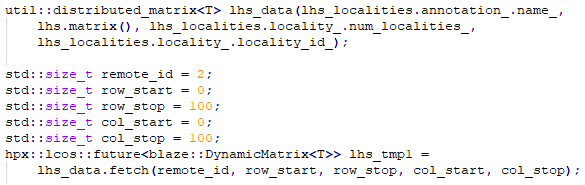
\includegraphics{dist_matrix_lhs}
	\caption{Phylanx distributed\_matrix example code}
	\label{Fig_1}
\end{figure}


As you can see, the distributed object exposes a fetch function which allows us to access non-local elements of the data structure in an object oriented way, using C++ Standard Library idioms (futures) similar to how one might access a data member of an ordinary local object. This convenient abstraction allows for distributed software development which is focused on the already difficult nature of structuring SPMD algorithms, instead of the nuts and bolts of remote data access. Another feature of the distributed\_object is that it is "lazy", in the sense that it registers itself with AGAS, and only finds the precise location of a colleague when that colleague's data is needed locally, and requested through the fetch function.
\paragraph{}
We were inspired to create Phylanx's distributed\_object by the UPC++ \cite{UPCXX} data structure of the same name. The main difference in its use is that Phylanx's distributed\_object requires a unique basename to be passed at construction in order for each local portion to find its non-local colleagues through HPX's Active Global Address Space (commonly referrred to as AGAS). Figure \ref{Fig_2} is sample code taken from the programmer's guide to UPC++  demonstrating the use of that library's version of a distributed\_object. 

\begin{figure}
	\centering
	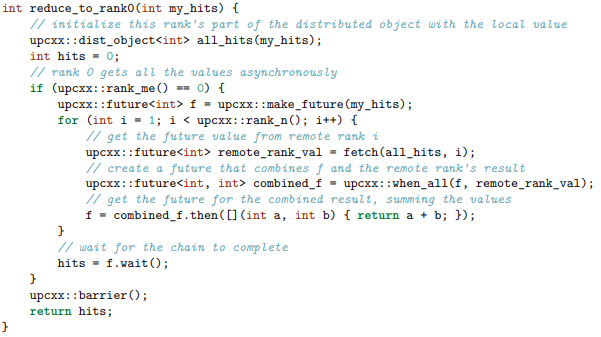
\includegraphics{dist_object_upcxx_example}
	\caption{UPC++ dist\_object example code}
	\label{Fig_2}
\end{figure}

\subsection{Tiling}
\paragraph{}
As mentioned previously, throughout our development of distributed functionality we had as one of our goals the eventual optimization of user-supplied programs with respect to tiling of distributed matrices. By tiling we mean the intentional distributed arrangement of data segments. For example, in the situation where we want to compute the matrix result $$A=B+C$$ on a set of four computational nodes, we could have many different arrangements of that data. Figure \ref{Fig_3} shows how each matrix involved must be intentionally allocated on a particular compute node in order for it to be used in the computation. Figure \ref{Fig_4} shows a non-optimal tiling (for our addition operation) which will require extra network communication (represented by arrows for the fetching) in order to compute the result. For matrix addition with uniform tiling the optimal solution is simple to find, as there is only one, when all corresponding tiles are co-located on one node. In the case of non-uniform tiling however, there is the possibility that even this optimal solution is not trivial to find, if blocks of A and B do not have an exact dimensional correspondence\footnote{This extra difficulty in finding an optimal set of tiling choices while non-uniform tiles are present is one reason why, although dot\_d allows us flexibility in this regard, we may not prefer to make use of it}.
\paragraph{}
For matrix addition, tiling decisions can be very easy. But for operations like matrix multiplication, there can be much greater complexity. Complicating factors include choice of algorithm, number of available processors, pre-existing tiling, as well as others. For instance, just in the algorithms we implemented, Cannon's algorithm requires a perfect square number of processors while dot\_d will function with any number of processors.  For situations with 35 available processors then, you may need to choose between the potential communication reduction benefits of tiling your matrices on 25 processors for compliance with Cannon's requirements, or trying to take advantage of all of the available processors with dot\_d. These are the sorts of questions we hoped developing more distributed functionality in Phylanx might help us answer, whether  we learn more in the design process or through the utilization of Phylanx as a testing environment.

\begin{figure}
	\centering
	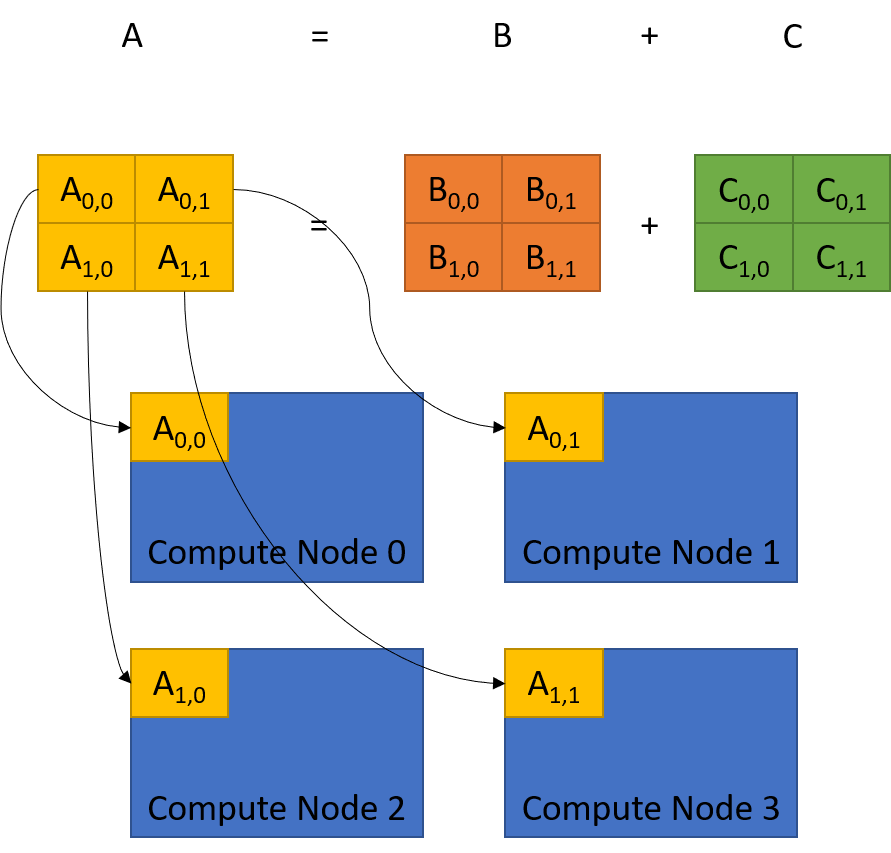
\includegraphics[width=100mm]{matrix_a_is_distributed}
	\caption{Creating a distributed object}
	\label{Fig_3}
\end{figure}

\begin{figure}
	\centering
	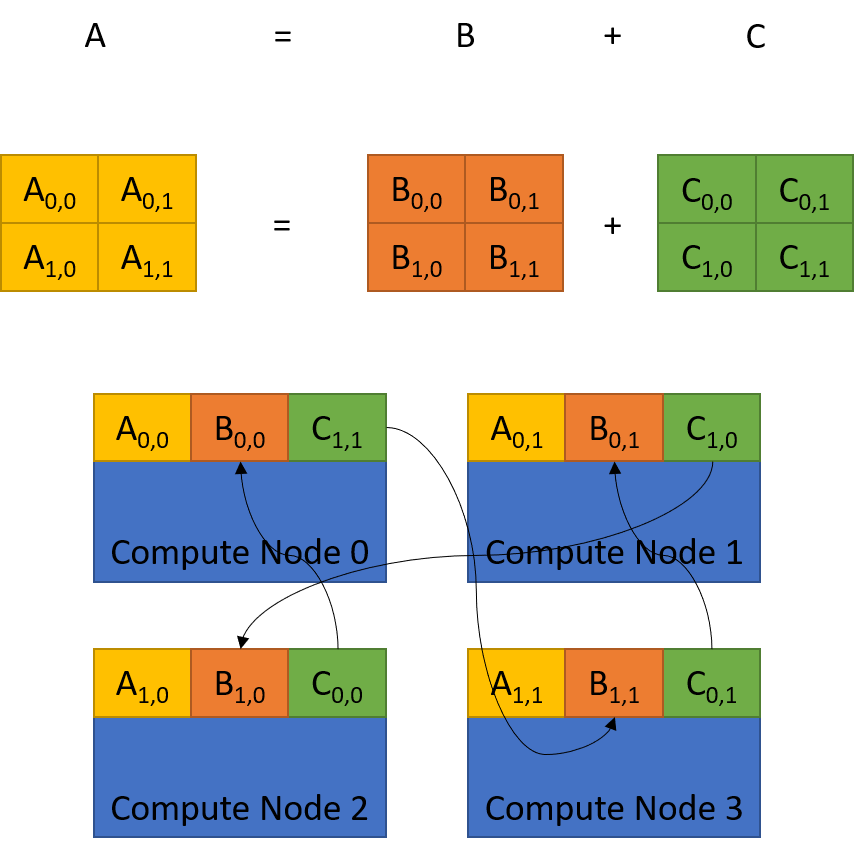
\includegraphics[width=100mm]{network_communication_fix_misalignment}
	\caption{Network communication required to address tiling mismatch}
	\label{Fig_4}
\end{figure}


\subsection{Annotations}
The data structure used to keep track of which blocks of each matrix are stored on which computational node is called the "annotation" in Phylanx. This is essentially a list of lists, which is established when the data structure is initially created, for example, when a matrix is loaded from disk and partitioned onto multiple nodes. At construction, the participating localities coordinate using AGAS, submitting their calculated share of the macro-level data structure, so that after every node has chimed in each node receives a copy of the annotations for the macro-level data structure. This means if the data structure, for example a matrix, is used in an algorithm, say multiplication, the node can find from the annotation which node owns the data it needs to progress in the calculation. Figure \ref{Fig_5} is an example of an annotation generated from a matrix of dimension 6x6 distributed across four localities. Again, each node stores a copy of this metadata, making it possible to identify the home node of any element in the macro-level matrix. 
\paragraph{}
It's important to note that while annotations are used in concert with the distributed\_matrix, the latter does not exist at all times. The underlying data, allocated locally on each node, persists as long as it is needed using RAII, and the distributed\_matrix behaves similarly. That is, the distributed\_matrix only exists as long as it is needed in the computation. Once the computation needing it is complete, it goes out of scope. Since the distributed object is "lazy", even if a matrix is distributed, and involved in many subsequent operations, each participating locality registers with AGAS only once per construction, and the IDs assigned by AGAS then are fetched as needed each time. Since all of these operations are occurring concurrently, with no object-wide barriers, this ensures that the program preserves its futurized nature (see chapter \ref{chap:cannon} for a discussion of futurization in AMTs). The annotations do still require a barrier on all participating localities at construction, in order for the annotation to be copied and distributed to each participating localities, but after that, the distributed\_matrix requires no further hard barriers unless the algorithm itself necessitates it. The operation of the distributed\_matrix was designed this way largely to avoid altering the most basic, persistent data-types in use in Phylanx, ensuring that they remained simpler shared memory data structures.

\begin{figure}
	\centering
	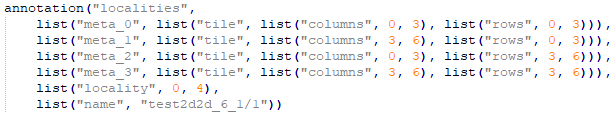
\includegraphics[width=100mm]{four_loc_annotation}
	\caption{Four node annotation}
	\label{Fig_5}
\end{figure}

\subsection{Summary}
\paragraph{}
The Phylanx project was started with the goal of producing a high-quality, performant package which would enable a simple pathway for domain scientists to port their programs to a distributed environment. Prerequisites for our work towards this goal have included development of distributed data structures, and representations for, as well as a system for better understanding, tiling. 



%

\pagebreak
\singlespacing
%%
%
\chapter{Conclusion}
\doublespacing
%

\label{chap:intro}
\paragraph{}
At the outset of this project we had several goals in mind. These included learning more about how to implement distributed primitives in the future, learning more about how to design these primitives with tiling in mind, and the actual development of two performant, distributed matrix multiplication algorithms. With respect to the first goal we now know that distributed primitives may need auxiliary data structures to support efficient organization of tiling information, and that writing distributed primitives is a process that is uniquely challenging, in a way that serial primitives is not. With respect to auxiliary data structures, an example is how we were required to construct a representation of the tile row from the annotation for the LHS operand and a representation of the tile column for the RHS operand in the Cannon Product. This is directly related to how the Cannon Product runs, and other algorithms may need their own tailored way of traversing existing tiling. In the case of dot\_d, we did not need an extra data structure for execution aside from the existing annotations. With respect to the second goal we learned that for tiling analysis with the goal of optimization, uniform tiling is much simpler to work with than non-uniform tiling. For the last goal, we produced two algorithms for matrix multiplication, as we set out to.
\section{Results}
With the two matrix multiplication algorithms completed, we were able to run some preliminary performance tests. Table \ref{table_1} displays those results in tabular form, and figure \ref{Fig_10} displays them in a graph. In figure \ref{Fig_11} we can see the speedup achieved by the respective algorithms, calculated as $Speedup = t_1/t_N$ where $t_1$ is the time in the single process version and $t_N$ is the version with $N$ processes. In our case, as they are only preliminary results, we only tested on 1 process, and on 4 processes. We obtained these results running the application with 4 separate processes on a single Windows machine, versus a single process for the linear version. Due to unexpected technical complications, we were not able to use the threading ordinarily used in the Blaze linear algebra library for our tests. Although our tests were performed in a shared memory environment, and thus could be contested, we believe that the requirement of communicating through the TCP/IP layer in HPX means that the results are approximately equivalent to running in a fully distributed environment. In the tests we ran, we found that the Cannon product was always the fastest, achieving a speed-up relative to the serial of between $~2.6$ and $~3.2$. Cannon consistently outperformed dot\_d. As we mentioned before, we believe that the lack of a reduction step across tile rows in the output matrix substantially aided the Cannon product, as well as its use of futurization of the fetches. Of course, further testing is required to confirm these results.


\begin{table}
	\centering
	\begin{tabular}{|c|c|c|c|} 
		\hline
		Matrix Size & dot\_d & Cannon & dot (serial) \\ [0.5ex] 
		\hline
		500 & 5351.08 & 3131.345 & 8538.37 \\ 
		\hline
		1000 & 26946.15 & 25889.2 & 67425.2 \\
		\hline
		2000 & 282916.5 & 170091.5 & 539491 \\ [1ex]
		\hline
	\end{tabular}
	\caption{Preliminary Test Results}
	\label{table_1}
\end{table}

\begin{figure}
	\centering
	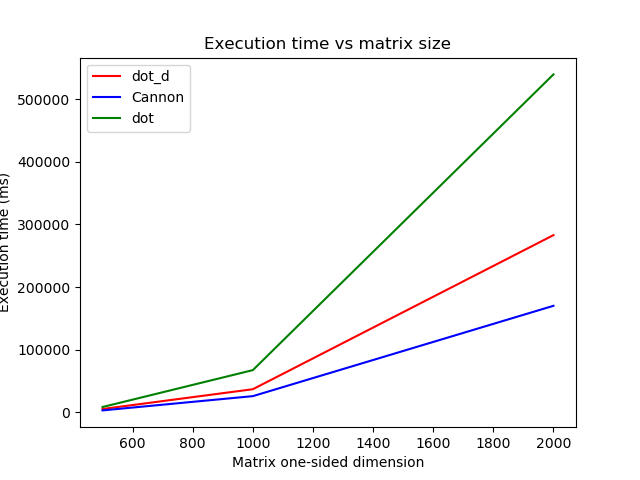
\includegraphics[width=150mm]{performance_comparison}
	\caption{Preliminary Test Results - Raw timings}
	\label{Fig_10}
\end{figure}

\begin{figure}
	\centering
	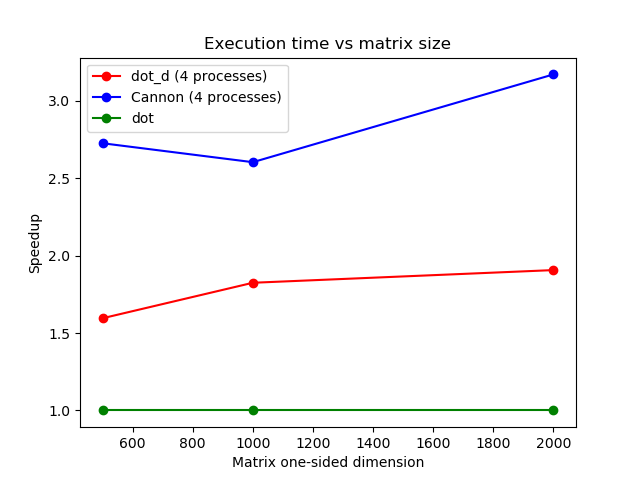
\includegraphics[width=150mm]{speed_up_plot}
	\caption{Preliminary Test Results - Speedup}
	\label{Fig_11}
\end{figure}

\section{Future work}
Although these results are only preliminary, they are encouraging, and suggest that our work on this project has meaningfully advanced the state of the Phylanx project. In order to advance closer to having a robust system for performing linear algebra for ML applications, or otherwise, we have several new objectives. The main one is in expanding our lineup of distributed primitives, to allow for something of a "distributed computational basis" for ML applications. This necessitates functionality like distributed add/map, distributed file read/write, and other linear algebra primitives like matrix inverse, and matrix factorization. We also would like to be able to use this system to aid in providing testing data for the tiling optimization facet of Phylanx. The capacity to write many different algorithms with different tilings, and extract performance data will help give intuition, or experimental validation, in the development of a static tiling optimizer.
	



%

\pagebreak
\singlespacing
%%
%%
%%To insert additional chapters, copy the previous five lines, using chapterX as the argument of the
%%\input command for Chapter X, where X=6,7,8,...
%% Adding appendix

%
\addtocontents{toc}{\vspace{12pt} \hspace{-1.8em} Appendix \vspace{-1em}}
%\addtocontents{toc}{\vspace{12pt} \hspace{-1.8em} Appendix \vspace{-1em}}
\appendix
\chapter{Supplementary Results}
\vspace{0.5em}
\label{app:supp}
If you have more than one appendix, this is the second one. 

  %%%%%%%%%%%%%%%%%%%%%%%%%%%%%%%%%%%%%%%%%%%%%%%%%%%%%%%%%%%%%%%%%%%%%%%%
  
  %

  


\pagebreak
\chapter{Copyright Information}
\vspace{0.5em}
\label{app:copyright}
This is the appendix for copyright information.
%%%%%%%%%%%%%%%%%%%%%%%%%%%%%%%%%%%%%%%%%%%%%%%%%%%%%%%%%%%%%%%%%%%%%%%%%%%%%%%%%%%%%%%%%%%

\pagebreak
%%If you need to insert additional appendices, copy the previous four lines, using appendixY as the
%%argument of the \input commnd for Appendix Y, for Y=C,D,E,...
%%
%%
%
\addtocontents{toc}{\vspace{12pt}}
\addcontentsline{toc}{chapter}{\hspace{-1.5em} {References}}
%
\bibliographystyle{unsrt}
\bibliography{references.bib}
\pagebreak
%%
%%%Finally, the vita section is created and included in the Table of Contents.
\chapter*{Vita}
\doublespacing
\vspace{0.2em}
\addtocontents{toc}{\vspace{12pt}}
\addcontentsline{toc}{chapter}{\hspace{-1.5em} {Vita}}
\label{chap:vita}
Maxwell Reeser received his Bachelor of Science in Computer Science in May 2018, from Louisiana State University. From 2018 to 2020 he pursued his MS in Computer Science at Louisiana State University while holding a student research position with the Ste||ar Group at LSU's Center for Computation and Technology where he was able to work on distributed data structures and primitives for the Phylanx Distributed Array Processing Toolkit project. He was also able to work on a variety of projects with Radiance Technologies including Python software development in graph algorithms and PySpark.


%%%%%%%%%%%%%%%%%%%%%%%%%%%%%%%%%%%%%%%%%%%%%%%%%%%%%%%%%%%%%%%%%%%%%%%%%%%%%%%%%%%%%%%%%%%

%%%%%%%%%%%%%%%%%%%%%%%%%%%%%%%%%%%%%%%%%%%%%%%%%%%%%%%%%%%%%%%%%%%%%%%%%%%%%%%%%%%%%%%%%%%

\end{document}
